\documentclass[a4paper]{article}

%% Language and font encodings
\usepackage[english]{babel}
\usepackage[utf8]{inputenc}
\usepackage[T1]{fontenc}

%% Sets page size and margins
\usepackage[a4paper,top=3cm,bottom=2cm,left=3cm,right=3cm,marginparwidth=1.75cm]{geometry}

%% Useful packages
\usepackage[tbtags]{amsmath}
\usepackage{mathtools}
\usepackage{graphicx}
\usepackage[colorinlistoftodos]{todonotes}
\usepackage[colorlinks=true, allcolors=blue]{hyperref}
\usepackage{color}
\usepackage{tikz}
\usepackage{titlesec}
\usepackage{caption}
\usepackage[shortlabels]{enumitem}
\usepackage{setspace}
\usepackage{authblk}
\usepackage{floatrow}

\floatstyle{plaintop}
\restylefloat{table}

\usetikzlibrary{shapes.geometric, arrows}

% package to manage citations
\usepackage[backend=bibtex,style=authoryear-comp,sorting=nyt,isbn=false,url=false, natbib=true, doi=false]{biblatex}
\addbibresource{bibliography.bib}

\tikzstyle{startstop_big} = [rectangle, rounded corners, minimum width=3cm, minimum height=1cm,text centered, draw=black,text width = 8.5cm, fill=red!30]
\tikzstyle{startstop} = [rectangle, rounded corners, minimum width=3cm, minimum height=1cm,text centered, draw=black,text width = 5cm, fill=red!30]
\tikzstyle{io} = [trapezium, trapezium left angle=70, trapezium right angle=110, minimum width=2cm, minimum height=1cm, text centered, draw=black, fill=blue!30]
\tikzstyle{process} = [rectangle, minimum width=3cm, minimum height=1cm, text centered, text width = 3cm, draw=black, fill=orange!30]
\tikzstyle{process_wide_3pt5cm} = [rectangle, minimum width=3cm, minimum height=1cm, text centered, text width = 3.5cm, draw=black, fill=orange!30]
\tikzstyle{process_wide_4cm} = [rectangle, minimum width=3cm, minimum height=1cm, text centered, text width = 4cm, draw=black, fill=orange!30]
\tikzstyle{process_wide_4pt5cm} = [rectangle, minimum width=3cm, minimum height=1cm, text width = 4.5cm, draw=black, fill=orange!30]
\tikzstyle{process_wide_5cm} = [rectangle, minimum width=3cm, minimum height=1cm, text width = 5cm, draw=black, fill=orange!30]
\tikzstyle{decision} = [diamond, minimum width=1cm, minimum height=1cm,text centered,text width = 2.25cm, draw=black, fill=green!30]
\tikzstyle{arrow} = [thick,->,>=stealth]


\definecolor{ErasmusBlue}{RGB}{12, 32, 116}

%Use 4 levels of sections using package titlesec
%\setcounter{secnumdepth}{4}
\newcommand{\subsubsubsection}[1]{\paragraph{#1}\mbox{}\\\\}
\newcommand*\diff{\mathop{}\!\mathrm{d}}
%\newcommand{\argmax}[1]{\underset{#1}{\operatorname{arg}\,\operatorname{max}}\;}
\DeclareMathOperator{\argmax}{arg\,max}
\DeclarePairedDelimiter\abs{\lvert}{\rvert}%
\DeclarePairedDelimiter\norm{\lVert}{\rVert}%

\let\bmath\boldsymbol
\let\rmn\mathrm
\newcommand{\Hline}
{
\hline
\hline
}


\begin{document}
\title{\textbf{Personalized Schedules for Kidney Transplant Patients}}

\author[1,*]{Firstname Lastname}
\affil[1]{Department of Biostatistics, Erasmus University Medical Center, the Netherlands}
\affil[ ]{*\textit {email}: a.tomer@erasmusmc.nl}

\date{}

\maketitle

%\doublespacing
% !TEX root =  ../ms.tex
\section{Introduction}
\label{sec : introduction}
According to the inclusion criteria of the study, a total of 239 kidney transplant patients were included in the data set. The transplantation characteristics of these patients is presented in Table \ref{tab : baseline_characteristics}. The data set also includes periodical measurements of serum creatinine (SCr) and protein creatinine ratio (PCR), which are biomarkers used to check the state of the transplant. The median number of repeated SCr and PCR measurements per patient are 45 and 37, respectively. For SCr 95\% of the observations are taken before 6 years, while for PCR they are taken before 5.4 years. The median time between two SCr measurements is 10 days, while the same for PCR is 14 days.

\begin{table}[!htb]
\begin{center}
\caption{Observed transplantation characteristics of the studied population (n = 239).}
\label{tab : baseline_characteristics}
\begin{tabular}{llr}
\Hline
\multicolumn{3}{c}{Quantitative characteristics} \\
\hline
Name & Abbreviation & Mean (SD) \\ 
\hline
Receiver age (at baseline) & rec\_age & 50.70 (13.09) \\
Donor age & d\_age & 49.73 (12.66) \\
Donor BMI & d\_bmi & 25.10 (4.43) \\
Receiver BMI & rec\_bmi & 25.43 (4.31) \\
Cold ischemia time (minutes) & cit & 887.25 (522.95)\\
\#HLA A, B and DR mismatches & hla & 2.81 (1.57)\\
Panel reactive antibody (\%) & pra & 4.81 (14.20) \\
\#Days on dialysis before transplant & dial\_days & 1334.91 (1283.93)\\
\#Anti-hypertensive medicaments & ah\_nr & 1.58 (0.96)\\
\hline
\\
\multicolumn{3}{c}{Categorical characteristics}\\
\hline
Name & Abbreviation & Category (\%) \\
\hline
Receiver gender & rec\_gender & Female (42.68 \%)\\
Donor gender & d\_gender & Female (56.49 \%)\\
Delayed graft function after transplant & dgf & No (67.78 \%)\\
Previous transplantation & prev\_tp & No (84.45 \%)\\
Diabetes mellitus & dm & No (84.52 \%)\\
Known cardiovascular events before transplant & hvdis & No (61.92 \%)\\
Deceased donor & d\_cadaveric & No (25.94 \%)\\
\hline     
\end{tabular}
\end{center}
\end{table}

In the cohort, 44 out of 239 patients observed graft failure (death-censored). The survival probability one year post transplantation is 97.87\%. The graft survival probabilities and 95\% CI estimated using Kaplan-Meier estimator are presented in Figure \ref{fig : km_curve}. 

\begin{figure}[!htb]
\centerline{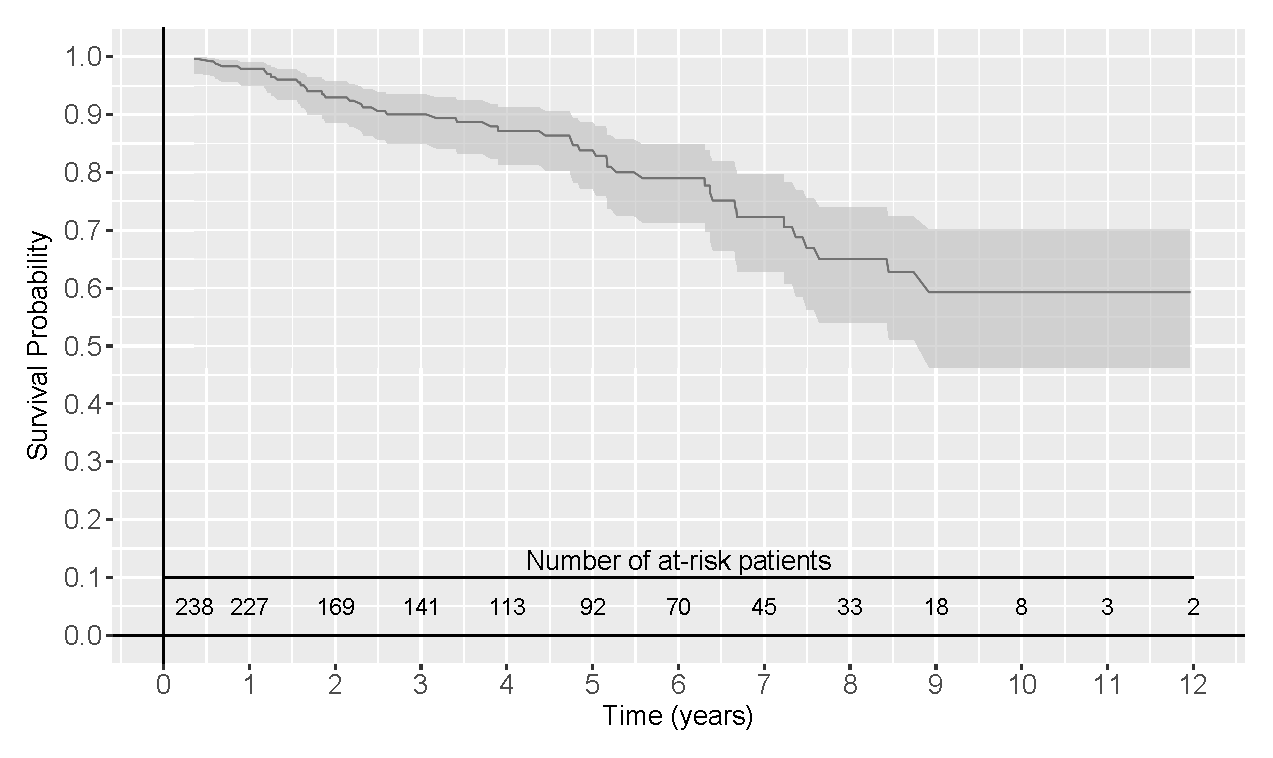
\includegraphics[width=\columnwidth]{images/km.eps}}
\caption{Graft survival probabilities and 95\% CI estimated using Kaplan-Meier estimator.}
\label{fig : km_curve}
\end{figure}

% !TEX root =  ../ms.tex

\section{Joint Model}
\label{sec : joint_model}
Our goal is to check if SCr and PCR both, are useful to predict graft failure. To this end, we model the two longitudinal outcomes and graft failure together using joint models (JMs) for time to event and longitudinal data \citep{tsiatis2004joint,rizopoulos2012joint}. In this model we use log transformed values of both SCr and PCR \citep{fournier2016joint}. More specifically, we model the impact of log(SCr) value and log(SCr) velocity, log(PCR) value and log(PCR) velocity, and transplantation characteristics on the hazard of graft failure. In this regard, the JM consists of a multivariate longitudinal sub-model to model the evolution of SCr and PCR and a relative risk sub-model to model the impact of transplantation characteristics and biomarkers on the hazard of graft failure. The longitudinal evolution of the two outcomes over time is modeled flexibly using B-splines. The model formulation for PCR outcome is as follows (for SCr outcome it is same):

\begin{equation}
\label{eq : long_model_prias}
\begin{aligned}
\log \mbox{PCR}(t) &= \beta_0 + \beta_1 \mbox{rec\_age} + \beta_2 \mbox{d\_age} + \beta_3 \mbox{d\_bmi} + \beta_4 \mbox{rec\_bmi} + \beta_5 \mbox{cit}\\
&+ \beta_6 \mbox{hla} + \beta_7 \mbox{pra}+ \beta_8 \mbox{dial\_days} + \beta_9 \mbox{ah\_nr} + \beta_{10} \mbox{rec\_gender} + \beta_{11} \mbox{d\_gender} \\
&+ \beta_{12} \mbox{dgf} + \beta_{13} \mbox{prev\_tp} + \beta_{14} \mbox{dm} + \beta_{15} \mbox{hvdis}+ \beta_{16} \mbox{d\_cadaveric}\\
&+\sum_{k=1}^4 \beta_{k+16} B_k(t,\mathcal{K}) +  b_{i0} + \sum_{k=1}^4 b_{ik} B_k(t,\mathcal{K}) + 
\varepsilon_i(t),
\end{aligned}
\end{equation}
where $B_k(t, \mathcal{K})$ denotes the $k$-th basis function of a B-spline with three internal knots at $\mathcal{K} =\{0.082, 0.219, 1\}$ (30 and 80 days recommended by the clinicians) years, and boundary knots at 0.039 and 6 years (minimum and 0.95 quantile of the time of measurements two outcomes). The quantitative transplantation characteristics are standardized to avoid convergence issues in parameter estimation. For the relative risk sub-model the hazard function we fit is given by:
\begin{equation}
\label{eq : hazard_prias}
h_i(t) = h_0(t) \exp\big\{\gamma_1 \mbox{prev\_tp} + \gamma_2 \mbox{hla}  + \gamma_3 \mbox{cit} + \gamma_4 \mbox{dial\_days} + \alpha_1 m_{i1}(t) + \alpha_2 m'_{i1}(t)\big\}.
\end{equation}
where $\alpha_1$ and $\alpha_2$ are measures of strength of the association between hazard of graft failure and $\log \mbox{PCR}$ value $m_{i1}(t)$ and $\log \mbox{PCR}$ velocity $m'_{i1}(t)$, respectively.

The parameters of the JM are estimated using the R package \textbf{JMbayes} \citep{rizopoulosJMbayes}, which uses the Bayesian methodology to estimate the model parameters (section B, supplementary material). Out of 239 patients, we use the data of only those 238 patients for whom both PCR and SCr data is available. The parameter estimates for the longitudinal sub-model for SCr and PCR are provided in Table \ref{tab : creatinine_long} and Table \ref{tab : pcr_long}, respectively. The effect of transplantation characteristics on both outcomes is small and ignorable, and hence not discussed in detail. Since the quantitative variables are standardized, the effect sizes correspond to one standard deviation increase in the corresponding variable. To avoid the tricky interpretation of variables corresponding to evolution over time, instead the evolution of SCr and PCR over time is depicted in Figure \ref{fig : creatinine_evolution}, and Figure \ref{fig : pcr_evolution}, respectively.
@Hessel: We have to explain why the creatinine levels dip. 

\begin{table}[!htb]
\begin{center}
\caption{Parameter estimates for the longitudinal model for SCr.}
\label{tab : creatinine_long}
\begin{tabular}{lrrrrr}
\Hline
Variable                                                                         & Mean   & Std. Dev & 2.5\%  & 97.5\% & P              \\
\hline
Intercept                                                                      & 5.226  & 0.080    & 5.064  & 5.378  & \textless0.000 \\
Receiver age                                                                   & -0.063 & 0.022    & -0.107 & -0.019 & 0.010          \\
Donor age                                                                          & 0.083  & 0.020    & 0.045  & 0.119  & \textless0.000 \\
Donor BMI                                                                          & -0.011 & 0.021    & -0.054 & 0.028  & 0.612          \\
Receiver BMI                                                                         & 0.018  & 0.023    & -0.025 & 0.060  & 0.420          \\
\#HLA mismatches between donor and recipient                                                                         & 0.020  & 0.022    & -0.022 & 0.065  & 0.342          \\
Panel reactive antibody percentage                                                                          & 0.048  & 0.027    & -0.008 & 0.100  & 0.082          \\
\#Anti-hypertensive medicaments                                                                           & 0.040  & 0.020    & 0.001  & 0.080  & 0.048          \\
Cold ischemia time                                                                         & 0.029  & 0.035    & -0.039 & 0.102  & 0.390          \\
\#Days on dialysis before transplant                                                                   & 0.015  & 0.029    & -0.042 & 0.071  & 0.580          \\
Receiver gender: Male                                                                     & 0.197  & 0.042    & 0.111  & 0.276  & \textless0.000 \\
Previous transplant: Yes                                                                & 0.016  & 0.064    & -0.115 & 0.141  & 0.786          \\
Donor gender: Male                                                                      & 0.053  & 0.042    & -0.027 & 0.136  & 0.198          \\
Delayed graft function: Yes                                                                       & 0.118  & 0.049    & 0.025  & 0.216  & 0.006          \\
Diabetes Mellitus: Yes                                                                        & -0.103 & 0.059    & -0.217 & 0.012  & 0.076          \\
Cardiovascular events before transplantation: Yes                                                                     & -0.047 & 0.043    & -0.129 & 0.044  & 0.272          \\
Deceased donor: Yes                                                                 & 0.163  & 0.082    & 0.004  & 0.313  & 0.044          \\
Spline: visit time [0.039, 0.082] years & -0.440 & 0.041    & -0.517 & -0.358 & \textless0.000 \\
Spline: visit time [0.082, 0.219] years & -0.182 & 0.053    & -0.284 & -0.081 & \textless0.000 \\
Spline: visit time [0.219, 1] years & -0.545 & 0.081    & -0.712 & -0.395 & \textless0.000 \\
Spline: visit time [1, 6] years & 0.007  & 0.083    & -0.155 & 0.176  & 0.946          \\
$\sigma$                                                                            & 0.190  & 0.001    & 0.187  & 0.192  & \\
\hline
\end{tabular}
\end{center}
\end{table}

\begin{table}[!htb]
\begin{center}
\caption{Parameter estimates for the longitudinal model for PCR.}
\label{tab : pcr_long}
\begin{tabular}{lrrrrr}
\Hline
              Variable                                                                   & Mean   & Std. Dev & 2.5\%  & 97.5\% & P              \\
              \hline
Intercept                                                                      & 3.731  & 0.179    & 3.398  & 4.083  & \textless0.000 \\
Receiver age                                                                   & 0.030  & 0.052    & -0.066 & 0.138  & 0.604          \\
Donor age                                                                          & 0.209  & 0.047    & 0.118  & 0.301  & \textless0.000 \\
Donor BMI                                                                          & -0.019 & 0.051    & -0.121 & 0.084  & 0.716          \\
Receiver BMI                                                                         & -0.116 & 0.050    & -0.219 & -0.021 & 0.014          \\
\#HLA mismatches between donor and recipient                                                                         & -0.013 & 0.049    & -0.112 & 0.086  & 0.776          \\
Panel reactive antibody percentage                                                                          & 0.047  & 0.061    & -0.066 & 0.166  & 0.446          \\
\#Anti-hypertensive medicaments                                                                           & 0.056  & 0.047    & -0.03  & 0.147  & 0.208          \\
Cold ischemia time                                                                         & 0.062  & 0.082    & -0.097 & 0.211  & 0.468          \\
\#Days on dialysis before transplant                                                                   & 0.006  & 0.066    & -0.120 & 0.134  & 0.952          \\
Receiver gender: Male                                                                     & -0.026 & 0.094    & -0.207 & 0.166  & 0.798          \\
Previous transplant: Yes                                                                & 0.035  & 0.149    & -0.241 & 0.332  & 0.816          \\
Donor gender: Male                                                                      & 0.114  & 0.096    & -0.079 & 0.303  & 0.228          \\
Delayed graft function: Yes                                                                       & 0.043  & 0.118    & -0.174 & 0.275  & 0.740          \\
Diabetes Mellitus: Yes                                                                        & 0.153  & 0.135    & -0.124 & 0.396  & 0.256          \\
Cardiovascular events before transplantation: Yes                                                                     & -0.016 & 0.106    & -0.221 & 0.199  & 0.890          \\
Deceased donor: Yes                                                                  & 0.144  & 0.193    & -0.246 & 0.509  & 0.462          \\
Spline: visit time [0.039, 0.082] years & -0.821 & 0.090    & -0.989 & -0.638 & \textless0.000 \\
Spline: visit time [0.082, 0.219] years & -0.578 & 0.131    & -0.838 & -0.304 & \textless0.000 \\
Spline: visit time [0.219, 1] years & -0.898 & 0.160    & -1.218 & -0.587 & \textless0.000 \\
Spline: visit time [1, 6] years & 0.460  & 0.234    & 0.015  & 0.927  & 0.036          \\
$\sigma$                                                                            & 0.479  & 0.004    & 0.472  & 0.486  & \\
\hline
\end{tabular}
\end{center}
\end{table}

\begin{figure}[!htb]
\centerline{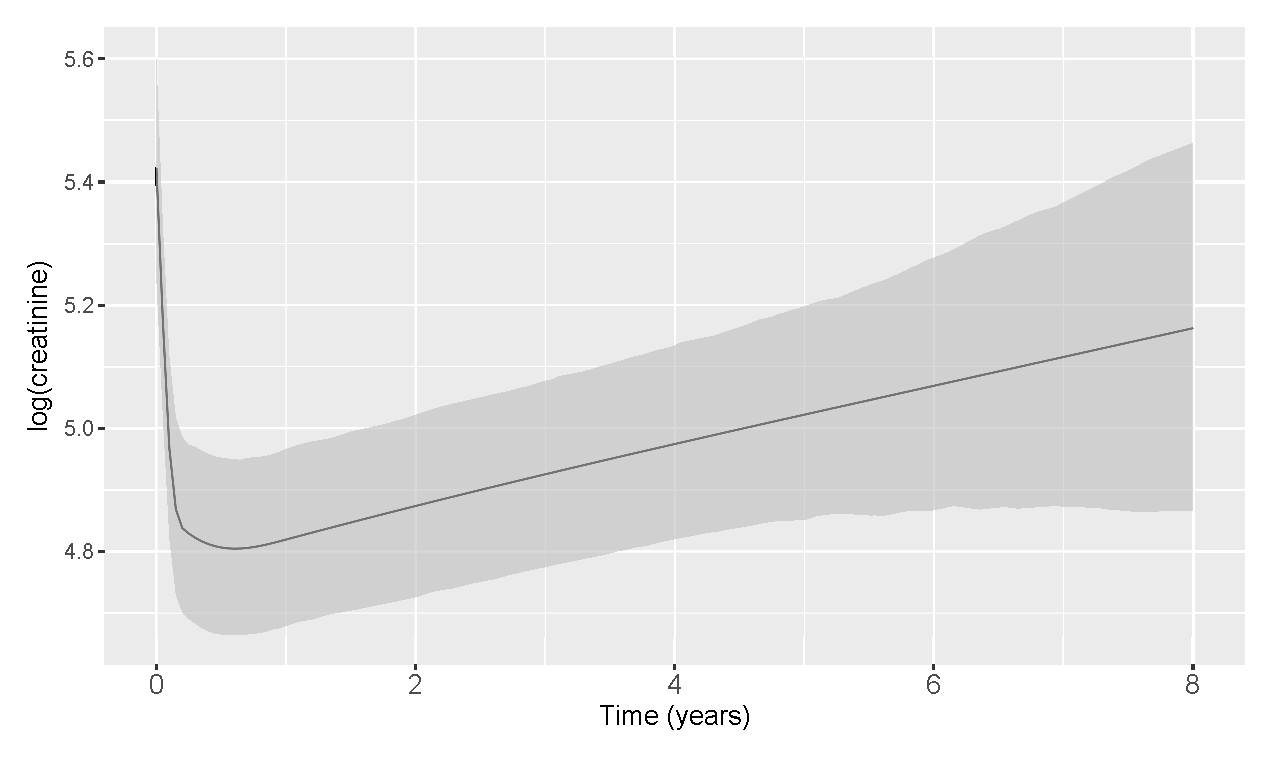
\includegraphics[width=\columnwidth]{images/creatinine.eps}}
\caption{Fitted longitudinal evolution of SCr and 95\% credible interval for a patient with the  transplantation characteristics described in Table \ref{tab : baseline_characteristics}.}
\label{fig : creatinine_evolution}
\end{figure}

\begin{figure}[!htb]
\centerline{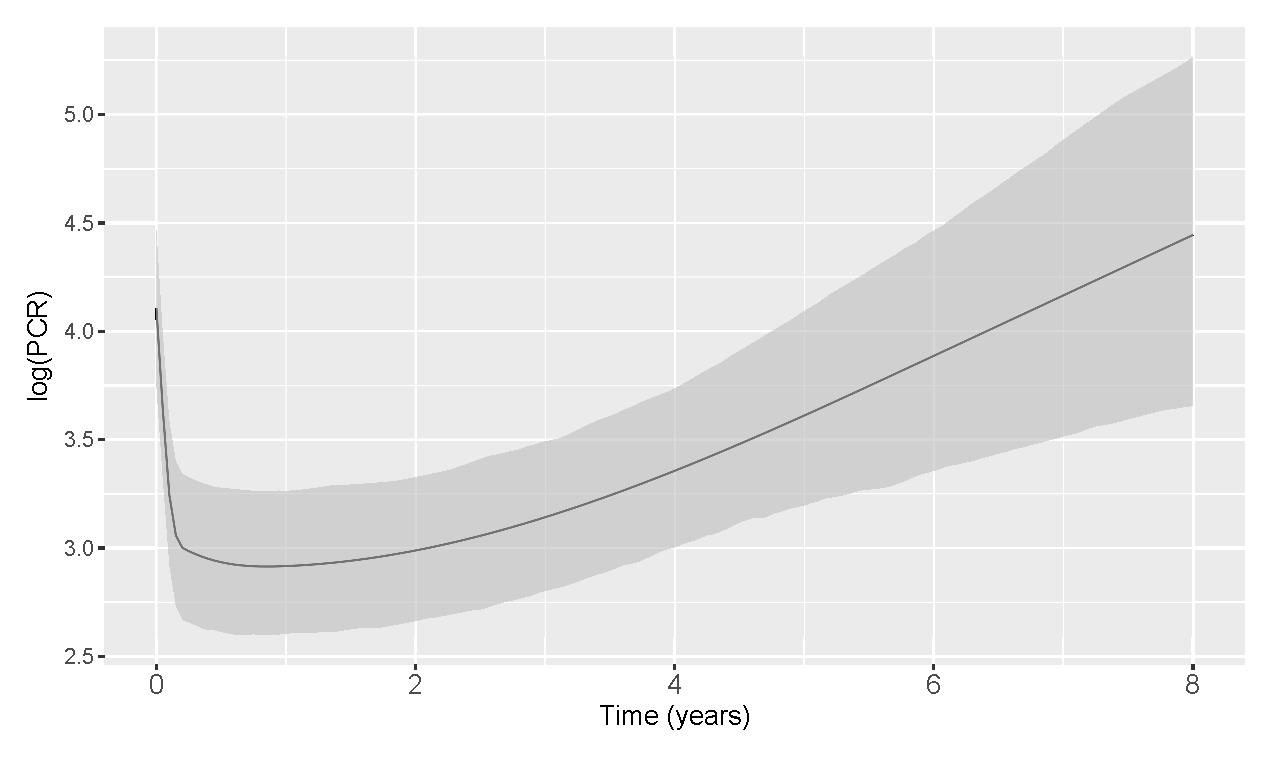
\includegraphics[width=\columnwidth]{images/pcr.eps}}
\caption{Fitted longitudinal evolution of PCR and 95\% credible interval for a patient with the  transplantation characteristics described in Table \ref{tab : baseline_characteristics}.}
\label{fig : pcr_evolution}
\end{figure}

The parameter estimates for the relative risk sub-model are provided in Table \ref{tab : relative_risk}. Since the quantitative variables are standardized, the effect sizes correspond to one standard deviation increase in the corresponding variable. We found that the $\log \mbox{SCr}$  levels are strongly associated with the hazard of GR. More specifically, for a given patient, if the SCr levels become twice and the remaining variables in the relative risk model remain the same, the hazard of graft failure increases three fold. $\log \mbox{PCR}$ levels and velocity are not strongly associated with hazard of GR. To further verify if they are required in the model in presence of both $\log \mbox{SCr}$ levels and velocity, we fitted two more JMs. In the first JM we modeled the association between $\log \mbox{SCr}$ levels and velocity and hazard of graft failure. In the second JM we modeled the association between $\log \mbox{PCR}$ levels and velocity and hazard of graft failure. We then calculated time dependent AUC, that is, area under the curve \citep{landmarking2017,rizopoulosJMbayes} values for all of the three JMs. The time dependent AUC were calculated periodically at an interval of 6 months. The first AUC was calculated at 6 months since transplantation and the last AUC was calculated at 3 years since transplantation. The resulting AUC values are plotted in Figure \ref{fig : auc_curve} and listed in Table \ref{tab : auc}. It can be seen that the model with both longitudinal outcomes performs the same as the model with only creatinine, to discriminate between patients who obtain graft failure versus others. Hence modeling PCR may not be necessary.

\begin{table}[!htb]
\begin{center}
\caption{Relative risk sub-model estimates for mean and 95\% credible interval.}
\label{tab : relative_risk}
\begin{tabular}{lrrrrr}
\Hline
Variable               & Mean   & Std. Dev & 2.5\%  & 97.5\% & P              \\
\hline
Previous transplant: Yes      & 0.305  & 0.339    & -0.099 & 0.986  & 0.352          \\
\#HLA mismatches between donor and recipient                & 0.048  & 0.093    & -0.114 & 0.269  & 0.620          \\
Cold ischemia time                & -0.051 & 0.105    & -0.277 & 0.133  & 0.644          \\
\#Days on dialysis before transplant         & -0.013 & 0.102    & -0.251 & 0.178  & 0.934          \\
$\log \mbox{PCR}$        & 0.145  & 0.125    & -0.056 & 0.431  & 0.188          \\
Slope($\log \mbox{PCR}$)        & 0.021  & 0.058    & -0.076 & 0.145  & 0.828          \\
$\log \mbox{SCr}$ & 1.599  & 0.241    & 1.067  & 2.063  & \textless0.000 \\
Slope($\log \mbox{SCr}$)  & 0.203  & 0.123    & -0.017 & 0.443  & 0.082  \\
\hline
\end{tabular}
\end{center}
\end{table}

\begin{figure}[!htb]
\centerline{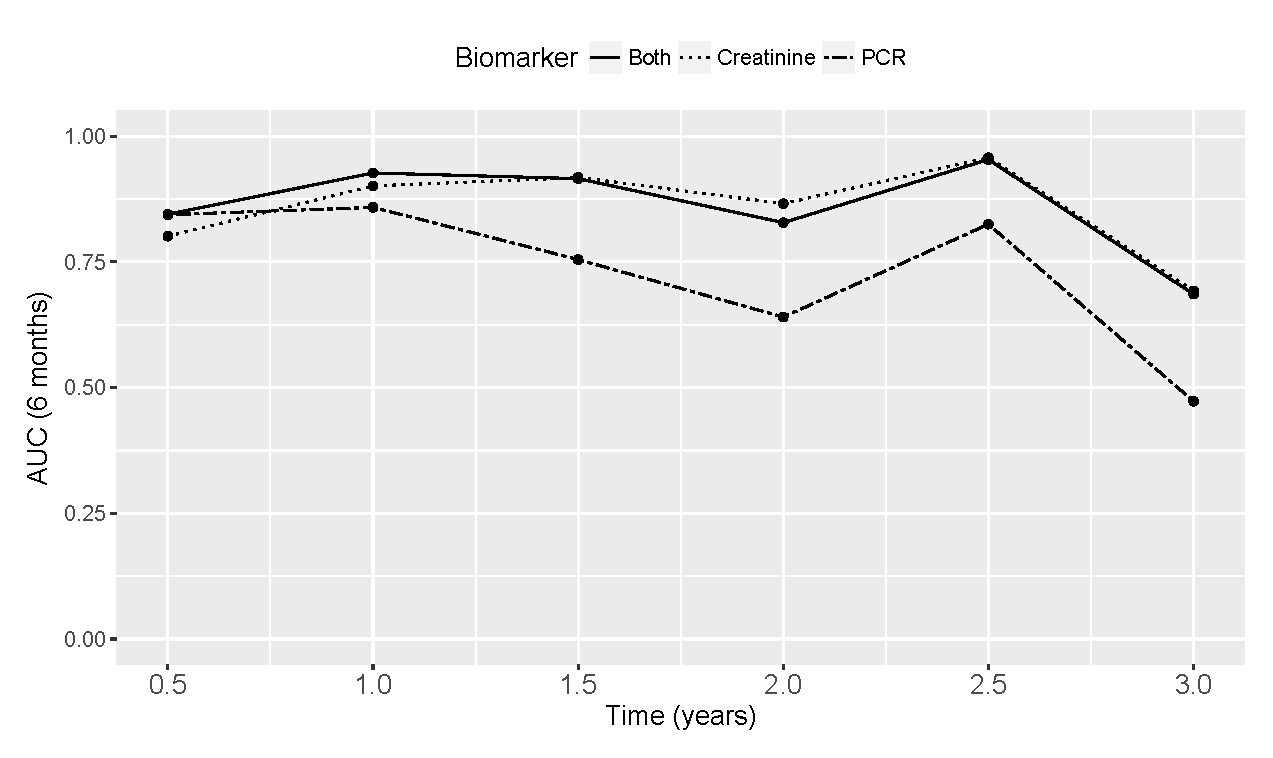
\includegraphics[width=\columnwidth]{images/auc.eps}}
\caption{Area under curve characteristics for the JMs fitted to the kidney transplant data set.}
\label{fig : auc_curve}
\end{figure}

\begin{table}[!htb]
\begin{center}
\caption{Area under curve characteristics for the JMs fitted to the kidney transplant data set.}
\label{tab : auc}
\begin{tabular}{lrrrrrr}
\Hline
Biomarkers               & Year 0.5   & Year 1 & Year 1.5  & Year 2 & Year 2.5 & Year 3 \\
\hline
Both SCr and PCR & 0.845 & 0.927 & 0.915 & 0.828 & 0.953 & 0.686\\
Only SCr & 0.801 & 0.901 & 0.918 & 0.866 & 0.957 & 0.692\\
Only PCR & 0.844 & 0.858 & 0.755 & 0.640 & 0.825 & 0.473\\
\hline
\end{tabular}
\end{center}
\end{table}
% !TEX root =  ../appendix.tex
\section{Personalized Schedules for Measurement of SCr}
\label{sec: simulation_study}
Currently, the schedule for measurement of SCr levels and fixed and common for all patients. SCr levels are measured 20 times in the first year after transplantation and every three months thereafter. Instead of a common fixed schedule for all patients, we propose using a different schedule for every patient. More specifically, we propose using personalized schedules based on joint models \citet{drizopoulosPersScreening}. Since the SCr measurements are already taken for the kidney transplant patients, in order to demonstrate the efficacy of the personalized schedules we conduct a small simulation. To this end, we first assume a population of kidney transplant patients, whose SCr and hazard of graft failure follow a JM of the form described in \ref{sec : jm_amctx}, with parameters equal to the posterior mean of parameters estimated from the joint model fitted to the kidney transplant dataset (Table \ref{tab : relative_risk_univariate} and Table \ref{tab : creatinine_long_univariate}). From this population we sample 625 patients, which are further split into a training (575 patients) and test (50 patients) part. For the training patients we generate a graft failure time $T^*_i$ as well as a random and non-informative censoring time $C_i$. For the test patients the graft failure time $T^*_j$ and an intervention time $T^I_j$ is generated. The intervention time is the time at which the 6 month dynamic risk of graft failure of the patient becomes larger than a certain threshold $\kappa$. The choice of $\kappa$ dictates the amount of time at hand between intervention and graft failure. In this simulation we evaluate two $\kappa$ values, namely 0.05 and 0.025. While the results for $\kappa = 0.05$ are presented in the main manuscript, here we present results for $\kappa = 0.025$. We fit a joint model of the specification described in Section \ref{sec : jm_amctx} to the training data set and obtain a MCMC sample from the posterior distribution of the parameters of the JM. Using the fitted JM, we then iteratively schedule SCr measurements for the test patients, until the dynamic risk of graft failure \citep{rizopoulos2011dynamic} of the patients becomes larger than the threshold $\kappa$. Let $N^I_j$ denote the number of SCr measurements conducted for the $j$-th test patient. The time difference between the observed intervention time due to the schedule ($T^S_j$) and the true intervention time, that is, the intervention offset is denoted by $O^I_j = T^S_j - T^I_j$. Lastly, the failure offset $O^*_j = T^S_j - T^*_j$ is the time at hand between the observed intervention time and the time of graft failure. Using the test patients, we calculate these measures for both personalized and fixed schedules. It is to be noted that in the ideal scenario, $N^I_j$ will be one, and offset $O^I_j$ will be zero. On the other hand ideally $O^*_j$ should be as small negative value as possible.

A boxplot of the observed values of the number of SCr measurements $N^I_j$, intervention offset $O^I_j$ and failure offset $O^*_j$ are presented in Figure \ref{fig : nObspt025}, Figure \ref{fig : truethrestimept025} and Figure \ref{fig : truestoptimept025}, respectively. An advantage of using 2.5\% risk over 5\% risk is that the risk of overshooting the true graft failure time is less due to less risk being taken. In this scenario, although the personalized schedule conducts less SCr measurements, it also exceeds the true intervention time more often than the fixed schedule.

\begin{figure}[!htb]
\centerline{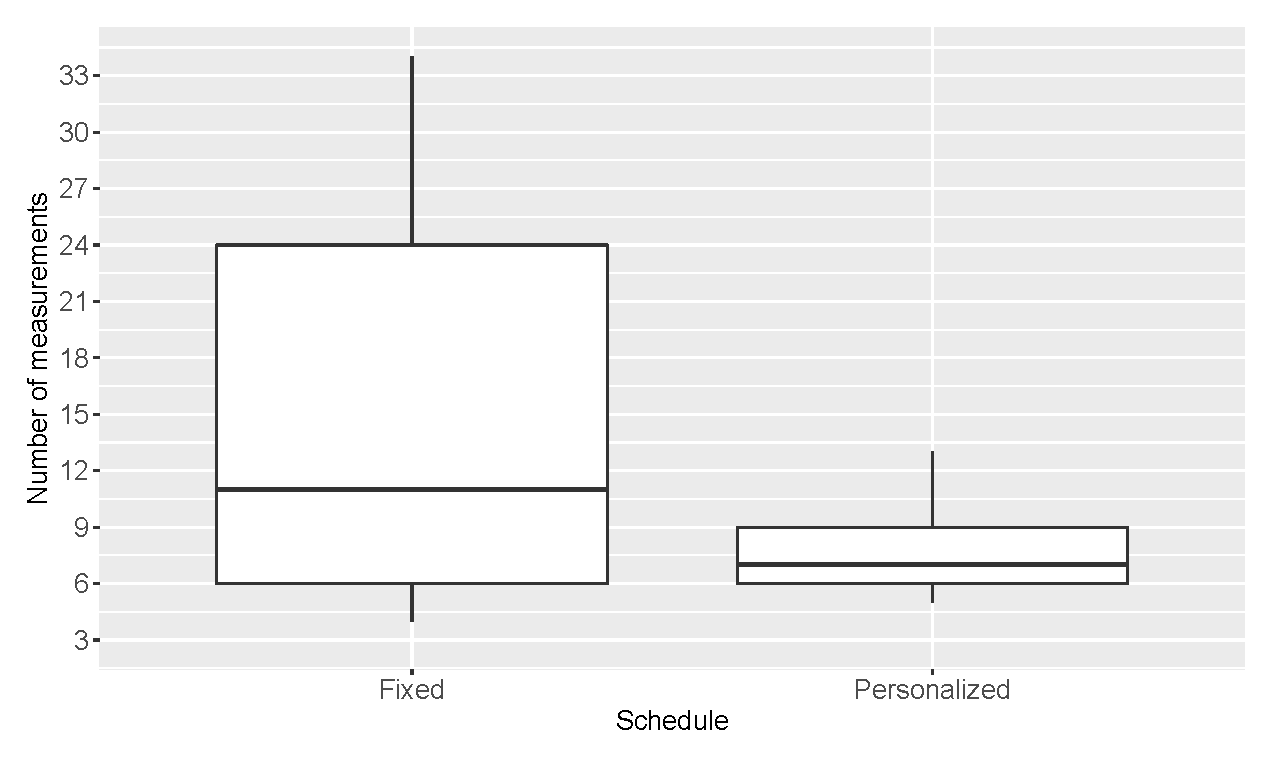
\includegraphics[width=\columnwidth]{images/nObspt025.eps}}
\caption{Boxplot of the number of SCr measurements $N^I_j$ for the test patients, for $\kappa = 0.025$.}
\label{fig : nObspt025}
\end{figure}

\begin{figure}[!htb]
\centerline{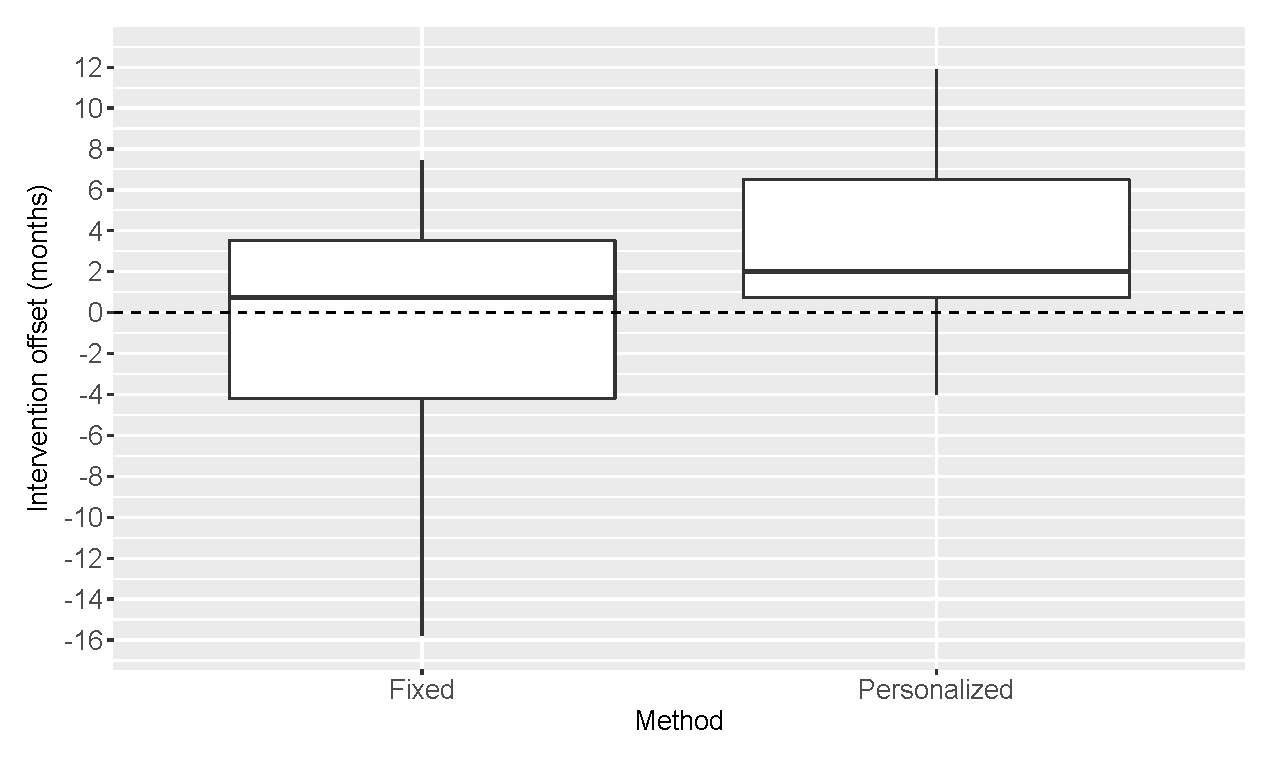
\includegraphics[width=\columnwidth]{images/truethrestimept025.eps}}
\caption{Boxplot of the intervention offset $O^I_j$ for the test patients, for $\kappa = 0.025$. The zero offset mark is displayed with the dashed line.}
\label{fig : truethrestimept025}
\end{figure}

\begin{figure}[!htb]
\centerline{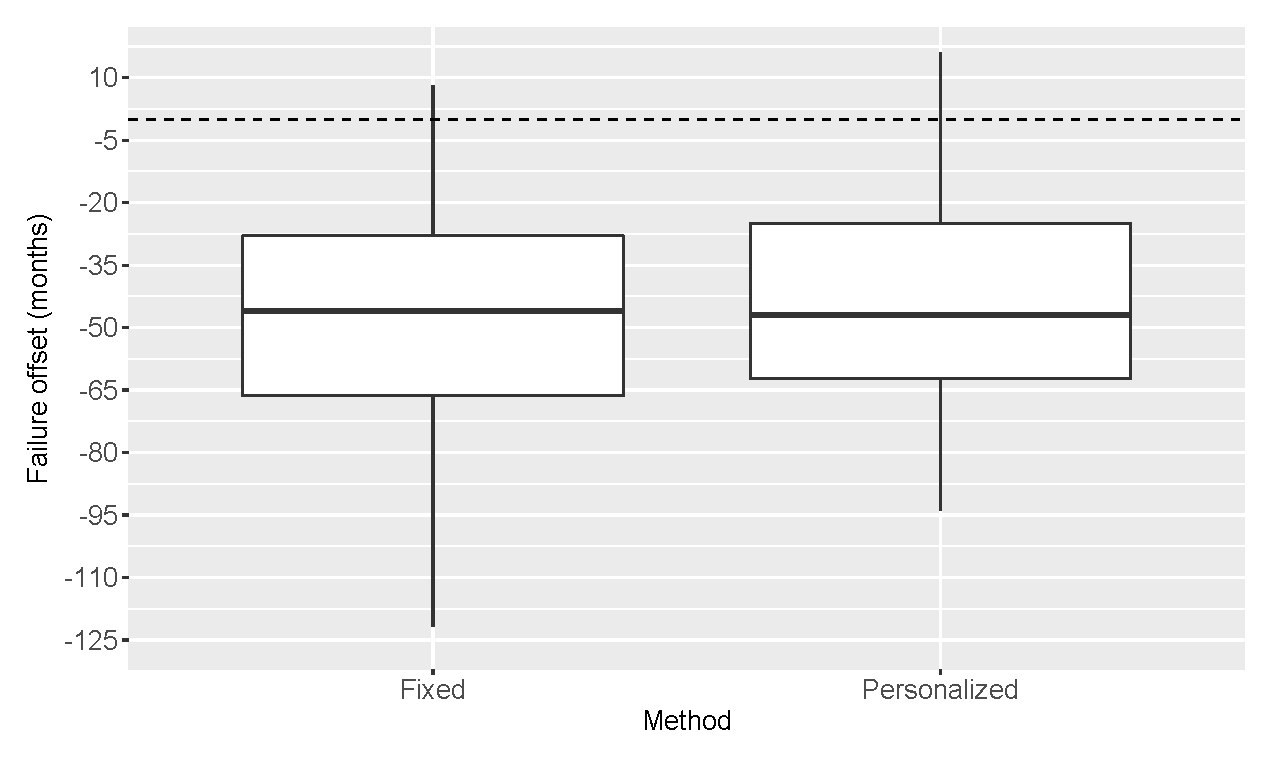
\includegraphics[width=\columnwidth]{images/truestoptimept025.eps}}
\caption{Boxplot of the failure offset $O^*_j$ for the test patients, for $\kappa = 0.025$. The zero offset mark is displayed with the dashed line.}
\label{fig : truestoptimept025}
\end{figure}


\textbf{}

\clearpage
\printbibliography

\appendix

\end{document}